%!TEX TS-program = xelatex
 
% Этот шаблон документа разработан в 2014 году
% Данилом Фёдоровых (danil@fedorovykh.ru) 
% для использования в курсе 
% <<Документы и презентации в \LaTeX>>, записанном НИУ ВШЭ
% для Coursera.org: http://coursera.org/course/latex .
% Исходная версия шаблона --- 
% https://www.writelatex.com/coursera/latex/5.2.2
 
\documentclass[a4paper,12pt]{article}
 
%%% Работа с русским языком
\usepackage[english,russian]{babel}   %% загружает пакет многоязыковой вёрстки
\usepackage{fontspec}      %% подготавливает загрузку шрифтов Open Type, True Type и др.
\defaultfontfeatures{Ligatures={TeX},Renderer=Basic}  %% свойства шрифтов по умолчанию
\setmainfont[Ligatures={TeX,Historic}]{Times New Roman} %% задаёт основной шрифт документа
\setsansfont{Comic Sans MS}                    %% задаёт шрифт без засечек
\setmonofont{Courier New}
\usepackage{indentfirst}
\frenchspacing
 
\renewcommand{\epsilon}{\ensuremath{\varepsilon}}
\renewcommand{\phi}{\ensuremath{\varphi}}
\renewcommand{\kappa}{\ensuremath{\varkappa}}
\renewcommand{\le}{\ensuremath{\leqslant}}
\renewcommand{\leq}{\ensuremath{\leqslant}}
\renewcommand{\ge}{\ensuremath{\geqslant}}
\renewcommand{\geq}{\ensuremath{\geqslant}}
\renewcommand{\emptyset}{\varnothing}
 
%%% Дополнительная работа с математикой
\usepackage{amsmath,amsfonts,amssymb,amsthm,mathtools} % AMS
\usepackage{icomma} % "Умная" запятая: $0,2$ --- число, $0, 2$ --- перечисление
 
%% Номера формул
%\mathtoolsset{showonlyrefs=true} % Показывать номера только у тех формул, на которые есть \eqref{} в тексте.
%\usepackage{leqno} % Нумерация формул слева
 
%% Свои команды
\DeclareMathOperator{\sgn}{\mathop{sgn}}
 
%% Перенос знаков в формулах (по Львовскому)
\newcommand*{\hm}[1]{#1\nobreak\discretionary{}
{\hbox{$\mathsurround=0pt #1$}}{}}
 
%%% Работа с картинками
\usepackage{graphicx}  % Для вставки рисунков
\graphicspath{{images/}{images2/}}  % папки с картинками
\setlength\fboxsep{3pt} % Отступ рамки \fbox{} от рисунка
\setlength\fboxrule{1pt} % Толщина линий рамки \fbox{}
\usepackage{wrapfig} % Обтекание рисунков текстом
 
%%% Работа с таблицами
\usepackage{array,tabularx,tabulary,booktabs} % Дополнительная работа с таблицами
\usepackage{longtable}  % Длинные таблицы
\usepackage{multirow} % Слияние строк в таблице
 
%%% Теоремы
\theoremstyle{plain} % Это стиль по умолчанию, его можно не переопределять.
\newtheorem{theorem}{Теорема}[section]
\newtheorem{proposition}[theorem]{Утверждение}
 
\theoremstyle{definition} % "Определение"
\newtheorem{corollary}{Следствие}[theorem]
\newtheorem{problem}{Задача}[section]
 
\theoremstyle{remark} % "Примечание"
\newtheorem*{nonum}{Решение}
 
%%% Программирование
\usepackage{etoolbox} % логические операторы
 
 
%%% Страница
\usepackage{extsizes} % Возможность сделать 14-й шрифт
\usepackage{geometry} % Простой способ задавать поля
	\geometry{top=5mm}
	\geometry{bottom=15mm}
	\geometry{left=5mm}
	\geometry{right=5mm}
 %
%\usepackage{fancyhdr} % Колонтитулы
% 	\pagestyle{fancy}
 	%\renewcommand{\headrulewidth}{0pt}  % Толщина линейки, отчеркивающей верхний колонтитул
% 	\lfoot{Нижний левый}
% 	\rfoot{Нижний правый}
% 	\rhead{Верхний правый}
% 	\chead{Верхний в центре}
% 	\lhead{Верхний левый}
%	\cfoot{Нижний в центре} % По умолчанию здесь номер страницы
 
\usepackage{setspace} % Интерлиньяж
%\onehalfspacing % Интерлиньяж 1.5
%\doublespacing % Интерлиньяж 2
%\singlespacing % Интерлиньяж 1
 
\usepackage{lastpage} % Узнать, сколько всего страниц в документе.
 
\usepackage{soul} % Модификаторы начертания
 
\usepackage{hyperref}
\usepackage[usenames,dvipsnames,svgnames,table,rgb]{xcolor}
\hypersetup{				% Гиперссылки
    unicode=true,           % русские буквы в раздела PDF
    pdftitle={Заголовок},   % Заголовок
    pdfauthor={Автор},      % Автор
    pdfsubject={Тема},      % Тема
    pdfcreator={Создатель}, % Создатель
    pdfproducer={Производитель}, % Производитель
    pdfkeywords={keyword1} {key2} {key3}, % Ключевые слова
    colorlinks=true,       	% false: ссылки в рамках; true: цветные ссылки
    linkcolor=red,          % внутренние ссылки
    citecolor=black,        % на библиографию
    filecolor=magenta,      % на файлы
    urlcolor=cyan           % на URL
}
 
\usepackage{csquotes} % Еще инструменты для ссылок
 
%\usepackage[style=authoryear,maxcitenames=2,backend=biber,sorting=nty]{biblatex}
 
\usepackage{multicol} % Несколько колонок
 
\usepackage{tikz} % Работа с графикой
\usepackage{pgfplots}
\usepackage{pgfplotstable}
 
\author{Батарин Егор}
\title{Изучение центрированных оптических систем}
\date{\today}
 
\begin{document} % конец преамбулы, начало документа
 
\maketitle
 
\begin{abstract}
    В работе используются: оптическая скамья, набор линз, экран, осветитель со шкалой, зрительная трубка, диафрагма, линейка
\end{abstract}
 
\section{Теория}
\begin{enumerate}
    \item Метод Аббе
        \begin{figure}[h!]
        \center{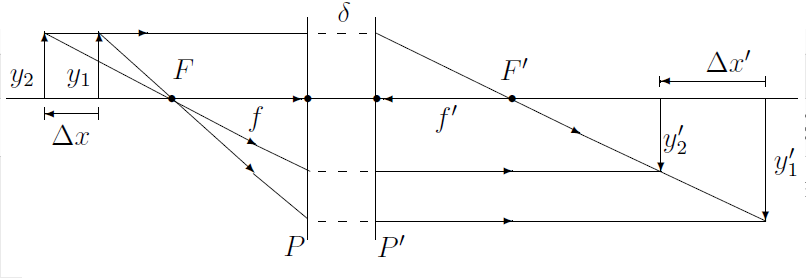
\includegraphics[scale = 0.7]{1.png}}
        \caption{Измерение фокусного расстояния по методу Аббе}
        \end{figure}
 
    Можно определить фокусное расстояние, перемещая предмет, по формуле \[f = \frac{\Delta{}x}{\Delta{}(y/y')} = \frac{\Delta{}x'}{\Delta{}(y'/y)}.\] 
    Для повышения точности стоит выбирать большие смещения, чтобы увеличение заметно отличалось
 
    \item Метод Бесселя
        \begin{figure}[h!]
        \center{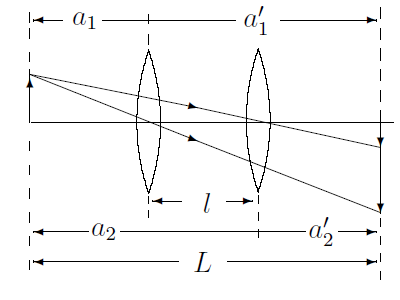
\includegraphics[scale = 0.9]{2.png}}
        \caption{Измерение фокусного расстояния по методу Бесселя}
        \end{figure}
 
    Итоговая используемая формула \[f = \frac{L^2 - l^2}{4L}.\] 
    То есть достаточно измерить L, l, при которых на экране видны чёткие изображения.
 
    \item Измерение фокусного расстояния тонкой собирающей линзы
    \[f = \frac{ab}{b + a}\]
 	\begin{figure}[h!]
 		\center{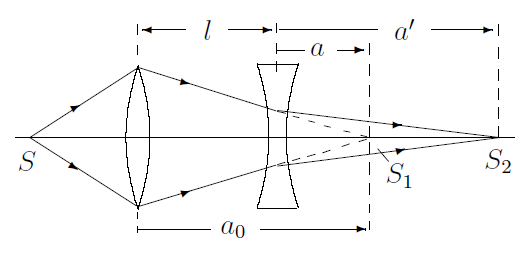
\includegraphics[scale = 1]{3.png}}
 		\caption{Фокусное расстояние для собирающей линзы}
 		
 		\[  f = l - a_0    \]
 	\end{figure}
    \item Сферическая аберация
        \begin{figure}[h!]
        \center{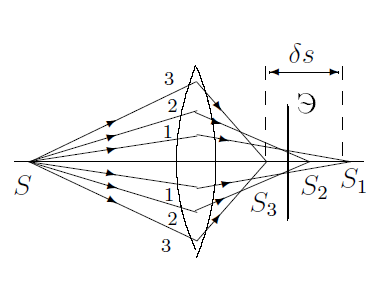
\includegraphics[scale = 1]{4.png}}
        \caption{Сферическая аберрация}
        \end{figure}
 
    Продольную аберацию линзы считаем, как \[\delta{}s(r) = s(r) - s(0).\]
 
    По наклону прямой далее найдём показатель преломления стекла линзы n.
 
 
\end{enumerate}
 
 
 
 
\section{Выполнение}
\begin{enumerate}
   \item Измерение фокусного расстояния по методу Абеля


Все расстояния измеряются в миллиметрах.
\begin{table}[h!]
	\begin{center}
	\begin{tabular}{|l|l|l|l|l|}
		\hline
		$\Delta{}x$&$\Delta{}x'$	& $y_1 = y_2$  & $y'_1$ & $y'_2$  \\ \hline
		365& 39 & 20 & 4 & 10 \\ \hline
	\end{tabular}
\end{center}
\end{table} 


Из данных таблицы по формуле Аббе получаем два значения для фокусных расстояний $f=127$ и $f'=130$.

Как видим, обе формулы дают похожие результаты, которые совпадают в пределах погрещностей.

\item Измерение фокусного расстояния рассеивающей линзы с помощью зрительной трубы.

В обеих случаях $a_0 = 420$. Для двух разных сторон получаем расстояния $l = 333$ и $l' = 329$. Для этих расстояний посчитаем соответсвующие фокусные расстояния $f = -87$, $f = - 91$.

\item Измерение фокусного расстояния сложной системы линз

\begin{table}[h!]
	\begin{center}
		\begin{tabular}{|l|l|l|l|l|}
			\hline
			$\Delta{}x$&$\Delta{}x'$	& $y_1 = y_2$  & $y'_1$ & $y'_2$  \\ \hline
			118& 71 & 20 & 9 & 28 \\ \hline
		\end{tabular}
	\end{center}
\end{table} 

Имеем соотвествующую таблицу для метода Аббе. Из нее получаем формулы для фокусных расстояний $f=78$ и $f'=75$. Можно сопоставить полученные значения с формулой для системы линз:
\[ \frac{1}{f_\text{сист}} = \frac{1}{f_1} + \frac{1}{f_2} - \frac{|l_{12}|}{f_1f_2}           \]

Из данной формулы получается значение $f_\text{сист} = 91$. Оно существенно отличается от значений выше. Причина заключается в неточном вычислении фокусных расстояний отдельных линз.

\item Нахождение положения главных фокусов линз

Для нахождения положения главного фокуса $F_{1\Sigma}$ будем передвигать осветитель так, чтобы получить резкое изображение предмета в окуляре зрительной трубы. Получим таким образом $F_{1\Sigma} = 69$. Далее переставим местами линзы, сохраняя расстояния между линзами $l_{12}$. Чтобы получить четкое изображение предмета, пришлось пододвинуть осветитель вплотную к первой линзе, поэтому можно сказать, что $0 \leq F_{2\Sigma} \leq 20$.

\section{Обсуждение погрешностей}

Данный эксперимент имеет определенное количество недостатков с точки зрения точности вычислений, выполненных на его основе:

1) Спектр света осветителя включает в себя довольно широкий диапазон частот, из-за чего, из-за дисперсии, нельзя точно определить, в каком месте находится резкое изображение предмета - возникает хроматическая аберрация. Эта ошибка порядка одного сантиметра.

2) Метка на осветителе была размазана, что доставляет погрешности при измерении размера предмета и изображения.

3) Линзы являются толстыми, потому нельзя точно определить необходимые расстояния, скажем, от предмета до линзы.

4) Форма линзы не является идеальной гиперболической - возникает сферическая аберрация.



Метод Аббе позволяет решить 3 проблему - в нем измеряются разности $\Delta{}x$ и $\Delta{}x'$, так что можно взять произвольную фиксированную точку на линзе и от нее отсчитывать расстояния - разница измеренных расстояний будет постоянна. Поскольку абсолютная погрешность значительно меньше измеренных расстояний, то относительная погрешность будет мала.



Метод Аббе, однако, не решает проблему 2, так как пришлось измерять абсолютные размеры стрелки и изображения. Он также не решает проблемы 1 и 4. Для решения решения проблемы 1, можно нанести на линзу пленочный фильтр, выделяющий монохроматический свет определенной частоты. Для решения проблемы 4, можно поставить на осветитель диафрагму и увеличить его яркость, чтобы изображение не было слишком тусклым. 


\end{enumerate}  
\end{document} % конец документа
 